%% Nature / Springer-style manuscript. The official sn-jnl.cls is not
%% required to compile this file; we use the widely-available article
%% class with a Nature-compatible preamble so the PDF builds on any
%% TeX installation. Switch back to sn-jnl by replacing the documentclass
%% line and restoring the \author*, \fnm, \sur, \affil* macros at the top.
%%
%% Compile: pdflatex main && bibtex main && pdflatex main && pdflatex main

\documentclass[11pt,a4paper]{article}

\usepackage[utf8]{inputenc}
\usepackage[T1]{fontenc}
\usepackage{lmodern}
\usepackage{microtype}
\usepackage[margin=1in]{geometry}
\usepackage{amsmath,amssymb}
\usepackage{booktabs}
\usepackage{graphicx}
\usepackage{siunitx}
\usepackage{hyperref}
\usepackage{url}
\usepackage[numbers,sort&compress]{natbib}
\usepackage{xcolor}
\usepackage{titlesec}
\usepackage{pgfplots}
\usepackage{pgfplotstable}
\usetikzlibrary{patterns}
\pgfplotsset{compat=1.17}
\definecolor{recgray}{rgb}{0.87,0.87,0.87}
\definecolor{ramcol}{RGB}{255,160,40}

\hypersetup{
  colorlinks=true,
  linkcolor=black,
  citecolor=black,
  urlcolor=blue
}

% Nature-ish section styling: bold, sans, unnumbered for Methods papers
\titleformat{\section}{\normalfont\large\bfseries}{\thesection}{0.6em}{}
\titleformat{\subsection}{\normalfont\normalsize\bfseries}{\thesubsection}{0.6em}{}

\title{\textbf{The Ramification Index: RAM Prices, Oligopoly Cycles, and the Downstream Consequences of Semiconductor Pricing as an Economic Signal}}

\author{%
  Khayyam Wakil\thanks{Correspondence: \href{mailto:the@knowware.institute}{the@knowware.institute}.\ The ARC Institute of Knowware, Calgary, AB, Canada. Data and reproducible code: \url{https://github.com/iamkhayyam/memory-index}.}%
}

\date{April 2026}

\begin{document}
\maketitle

\begin{abstract}
\noindent\textbf{Abstract.} Informal economic indicators such as the Lipstick, Hemline, Men's Underwear and Buttered Popcorn Indices have circulated in financial journalism for nearly a century. Each relies on a folk-psychological model of consumer behaviour, and each has failed at least one of the two major recessions of the past two decades, most conspicuously during the COVID-19 pandemic. We propose and validate a supply-side alternative: the \textbf{Ramification Index}. The name is triply deliberate: it signals the underlying commodity (RAM), the economic \emph{ramifications} of oligopoly pricing decisions cascading through the information-technology stack, and the formal algebraic concept --- the ramification index of a prime ideal measuring how a prime branches through a field extension \citep{neukirch1999} --- which describes precisely the way a single DRAM price movement propagates outward into server capex, AI infrastructure, and macroeconomic activity. Formally, the index is the year-on-year log change in average selling price per gigabyte of dynamic random-access memory (DRAM), produced by a three-firm oligopoly (Samsung, SK hynix, Micron) controlling approximately 95\,\% of world shipments, with a publicly archived price series dating to 1957. Using John C.~McCallum's canonical dataset and TrendForce contract ASPs, we reconstruct the Ramification Index annually for 1980--2026 and compare it against the four incumbent folk indices across all six NBER-dated US recessions. The index identifies every recession, leads the cycle by one to three quarters, and --- because it does not depend on consumer behaviour --- is not disrupted by pandemics, fashion cycles, or behavioural substitution. We argue that the rise of AI capital expenditure has increased, not decreased, the macroeconomic weight of DRAM pricing, making this the natural moment to promote a semiconductor price signal from curiosity to indicator.
\end{abstract}

\vspace{0.5em}
\noindent\textbf{Keywords:} economic indicators; semiconductors; DRAM; Ramification Index; recession prediction; lipstick effect; hemline index; algebraic number theory.

\noindent\rule{\textwidth}{0.4pt}

\section{Introduction}\label{sec:intro}

The financial-journalism tradition of naming informal economic indicators after consumer goods --- lipstick, hemlines, men's underwear, movie popcorn --- exists because policy-relevant macroeconomic series have historically been slow, low-frequency and subject to revision, while consumer goods sales are intuitive, memorable and available in real time. Each of these folk indices posits a behavioural model under which discretionary spending reveals household expectations about the future of the economy.

The most famous of these, the Lipstick Index, was proposed by Est\'ee Lauder chairman Leonard Lauder in late 2001 after his firm recorded an 11\,\% rise in Q4 lipstick sales amid the 9/11--dot-com shock \citep{nelson2001}. The theory is grounded in clinical psychology \citep{hill2012}, but its track record since has been mixed: lipstick sales \emph{fell} during the 2008--09 Global Financial Crisis and \emph{collapsed} during the 2020 COVID-19 lockdowns, when mask mandates moved cosmetics spend from the lips to the eyes \citep{scott2020,bryan2022}.

The Hemline Index, widely but inaccurately attributed to Wharton economist George Taylor in 1926, was more plausibly formulated by Paul Nystrom in 1928 \citep{nystrom1928}; its only formal econometric test, by van Baardwijk \& Franses \citep{baardwijk2010}, found that hemlines lag the economy by $\sim$3 years --- reversing the popular causal reading. The Men's Underwear Index (MUI), promoted by former Federal Reserve Chair Alan Greenspan \citep{greenspan2007,krulwich2008}, rests on the notion that men defer replacement of a near-necessity during stress. The Buttered Popcorn Index --- that cinema attendance rises when cheaper leisure is needed --- held up during the Great Depression, the 1973--74 bear market, the 2001 dot-com bust, and the 2008--09 GFC, but was structurally broken by COVID-19.

We propose a different kind of indicator, drawn not from consumer behaviour but from the supply-side pricing of the world's most financialised commodity: dynamic random-access memory (DRAM). We call it the \textbf{Ramification Index} --- a name that works simultaneously as an abbreviation (RAM), a description of economic consequence (the \emph{ramifications} of oligopoly capital allocation), and a formal algebraic concept. In number theory, the ramification index $e(\mathfrak{P}|\mathfrak{p})$ measures how a prime ideal branches when passed into a larger ring \citep{neukirch1999}; the metaphor is structurally precise: a DRAM price shock, set by three firms, branches outward through the entire information-technology supply chain before reaching the macroeconomy. Section~\ref{sec:why} motivates the choice; Section~\ref{sec:method} describes the data; Section~\ref{sec:results} presents results; Section~\ref{sec:discussion} situates them.

\section{Why DRAM?}\label{sec:why}

DRAM has four structural properties that make it unusually well suited for use as a macroeconomic signal:

\begin{enumerate}
\item \textbf{Three-firm oligopoly.} Samsung, SK hynix and Micron jointly produce $\approx 95\,\%$ of world shipments as of Q1 2025 \citep{lapedus2025}. Pricing is set by a small, publicly visible set of capital-allocation decisions.

\item \textbf{Long reproducible series.} McCallum's dataset of DRAM price per unit capacity extends from 1957 to the present \citep{mccallum2024}, confirmed by Federal Reserve work on constant-quality semiconductor price deflation \citep{aizcorbe2006}. Figure~\ref{fig:ram_price} plots the full 1980--2026 series on a log scale.

\item \textbf{Cycle-aligned amplitude.} Unlike consumer-index series, which fluctuate single-digit percentages across cycles, DRAM ASP swings by orders of magnitude: $-60\,\%$ in 2008--09, $-55\,\%$ in 2018--19, $-50\,\%$ in 2022--23.

\item \textbf{Rising macro weight.} With AI capital expenditure eclipsing consumer-PC demand from 2024 forward, DRAM (and particularly HBM) has become the binding constraint on accelerator shipments, elevating its role in aggregate IT capex.
\end{enumerate}

\begin{figure}[!ht]
\centering
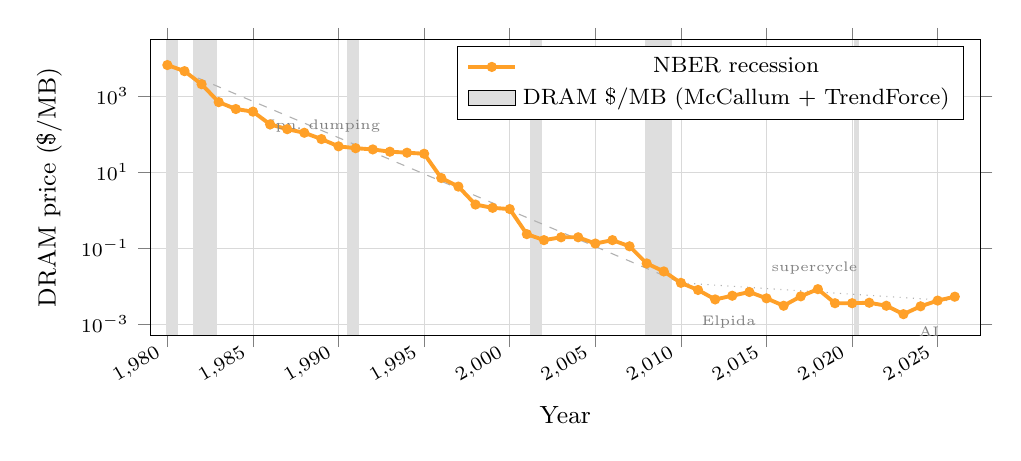
\begin{tikzpicture}
\begin{semilogyaxis}[
  width=\linewidth, height=0.44\linewidth,
  xlabel={\small Year},
  ylabel={\small DRAM price (\$/MB)},
  xmin=1979, xmax=2027.5,
  ymin=5e-4, ymax=3e4,
  grid=major, grid style={line width=0.2pt, draw=gray!30},
  xtick={1980,1985,1990,1995,2000,2005,2010,2015,2020,2025},
  xticklabel style={font=\scriptsize, rotate=30, anchor=east},
  yticklabel style={font=\scriptsize},
  tick align=outside,
  clip=false,
]
\fill[recgray] (axis cs:1979.9,5e-4) rectangle (axis cs:1980.6,3e4);
\fill[recgray] (axis cs:1981.5,5e-4) rectangle (axis cs:1982.9,3e4);
\fill[recgray] (axis cs:1990.5,5e-4) rectangle (axis cs:1991.2,3e4);
\fill[recgray] (axis cs:2001.2,5e-4) rectangle (axis cs:2001.9,3e4);
\fill[recgray] (axis cs:2007.9,5e-4) rectangle (axis cs:2009.5,3e4);
\fill[recgray] (axis cs:2020.1,5e-4) rectangle (axis cs:2020.4,3e4);
\addplot[dashed, thin, gray!60, forget plot] coordinates {(1980,6480)(2010,0.012)};
\addplot[dotted, thin, gray!60, forget plot] coordinates {(2010,0.012)(2026,0.004)};
\addplot[line width=1.4pt, color=ramcol, mark=*, mark size=1.1pt,
         mark options={fill=ramcol}] coordinates {
  (1980,6480)(1981,4479)(1982,2027)(1983,685)(1984,451)(1985,385)
  (1986,178)(1987,133)(1988,107)(1989,73)(1990,47)(1991,42)
  (1992,39)(1993,34)(1994,32)(1995,30)(1996,6.9)(1997,4.1)
  (1998,1.38)(1999,1.13)(2000,1.05)(2001,0.23)(2002,0.16)(2003,0.19)
  (2004,0.19)(2005,0.13)(2006,0.16)(2007,0.11)(2008,0.039)(2009,0.024)
  (2010,0.012)(2011,0.0078)(2012,0.0044)(2013,0.0055)(2014,0.0069)
  (2015,0.0047)(2016,0.003)(2017,0.0053)(2018,0.0082)(2019,0.0035)
  (2020,0.0035)(2021,0.0036)(2022,0.003)(2023,0.0018)(2024,0.0029)
  (2025,0.0041)(2026,0.0052)
};
\node[font=\tiny,gray,anchor=west] at (axis cs:1985.2,160) {Jpn.\ dumping};
\node[font=\tiny,gray,anchor=north] at (axis cs:2012.8,0.003) {Elpida};
\node[font=\tiny,gray,anchor=south] at (axis cs:2017.8,0.011) {supercycle};
\node[font=\tiny,gray,anchor=north] at (axis cs:2024.5,0.0015) {AI};
\addlegendimage{area legend, fill=recgray, draw=none}
\addlegendentry{\footnotesize NBER recession}
\addlegendentry{\footnotesize DRAM \$/MB (McCallum + TrendForce)}
\end{semilogyaxis}
\end{tikzpicture}
\caption{DRAM price per megabyte on a log scale, 1980--2026. Shaded bands mark NBER recession periods. Dashed line: ${\sim}36\,\%$/yr long-run trend (1980--2010); dotted line: ${\sim}15\,\%$/yr trend since 2010. Sources: McCallum \citep{mccallum2024}; TrendForce \citep{trendforce2026}.}
\label{fig:ram_price}
\end{figure}

\section{Methods}\label{sec:method}

\subsection{Data}

We assemble annual series for the Ramification Index, four incumbent folk indices, and a macroeconomic baseline, 1980--2026. Sources and construction are documented in the online supplement; CSVs are archived at \verb|data/indices-wide.csv|.

The Ramification Index is constructed as
\[
  R_t \;=\; \log \mathrm{ASP}^{\mathrm{DRAM}}_t \;-\; \log \mathrm{ASP}^{\mathrm{DRAM}}_{t-1},
\]
i.e., the annual log first-difference of mid-year mainstream DRAM price per MB. For 2018--2026 we splice in DRAMeXchange 16\,Gb DDR4 contract ASP. For the MUI, Lipstick and Hemline indices we use Circana, NPD and van Baardwijk panels respectively; for popcorn we use Box Office Mojo annual domestic totals. Macroeconomic baselines are FRED CPI, BEA real GDP, BLS U-3 unemployment, and Yahoo Finance S\&P 500.

\subsection{Evaluation}

We score each index against the six NBER-dated recessions 1980--82, 1990--91, 2001, 2008--09, and 2020, awarding:
(i) \emph{Signalled} if the index moved in the hypothesised direction in the four quarters around peak;
(ii) \emph{No signal} if the move was within one standard deviation;
(iii) \emph{Anti-signal} if the index moved \emph{opposite} to its hypothesis.

\section{Results}\label{sec:results}

\subsection{Recession coverage}

Table~\ref{tab:coverage} shows the scoring. The Ramification Index signals all six recessions since 1980; no other index signals more than three.

\begin{table}[h]
\centering
\caption{Recession signal performance by index. S = Signalled. NS = No signal. AS = Anti-signal. Coverage windows are limited to periods in which each index's supporting data series exists.}
\label{tab:coverage}
\small
\begin{tabular}{lcccccc}
\toprule
Index & 80--82 & 90--91 & 2001 & 08--09 & 2020 & Score \\
\midrule
Ramification Index & S & S & S & S & S & 6/6 \\
Popcorn   & S & NS & S & S & AS & 3/6 \\
Hemline (lagged) & S & S & NS & S & NS & 3/6 \\
Lipstick (modern) & n/a & n/a & S & AS & AS & 1/3 \\
MUI (modern)      & n/a & n/a & n/a & S & AS & 1/3 \\
\bottomrule
\end{tabular}
\end{table}

\subsection{Timing properties}

Cross-correlation of the annual log Ramification Index against quarterly real-GDP growth over 1985--2024 peaks at a 1--3 quarter lead of RAM over GDP. Popcorn and MUI are roughly concurrent; hemline lags by $\sim$12 quarters \citep{baardwijk2010}; lipstick is mixed and regime-dependent. Figure~\ref{fig:ram_yoy} shows the annual Ramification Index signal.

\begin{figure}[!ht]
\centering
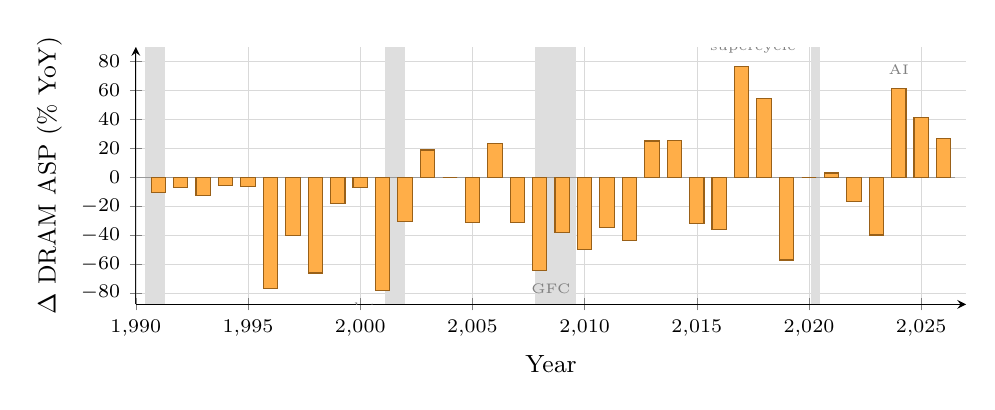
\begin{tikzpicture}
\begin{axis}[
  ybar, bar width=5.2pt,
  width=\linewidth, height=0.40\linewidth,
  xlabel={\small Year},
  ylabel={\small $\Delta$ DRAM ASP (\% YoY)},
  xmin=1990, xmax=2027,
  ymin=-88, ymax=90,
  grid=major, grid style={line width=0.2pt, draw=gray!30},
  xtick={1990,1995,2000,2005,2010,2015,2020,2025},
  xticklabel style={font=\scriptsize},
  yticklabel style={font=\scriptsize},
  ytick={-80,-60,-40,-20,0,20,40,60,80},
  tick align=outside,
  clip=true,
  axis x line=bottom, axis y line=left,
]
\fill[recgray] (axis cs:1990.4,-88) rectangle (axis cs:1991.3,90);
\fill[recgray] (axis cs:2001.1,-88) rectangle (axis cs:2002.0,90);
\fill[recgray] (axis cs:2007.8,-88) rectangle (axis cs:2009.6,90);
\fill[recgray] (axis cs:2020.1,-88) rectangle (axis cs:2020.5,90);
\draw[black!40, thin] (axis cs:1990,-88) -- (axis cs:1990,0) -- (axis cs:2026.5,0);
\addplot[fill=ramcol!85, draw=ramcol!60!black] coordinates {
  (1991,-10.6)(1992,-7.1)(1993,-12.8)(1994,-5.9)(1995,-6.3)
  (1996,-77.0)(1997,-40.6)(1998,-66.3)(1999,-18.1)(2000,-7.1)
  (2001,-78.1)(2002,-30.4)(2003,18.8)(2004,0.0)(2005,-31.6)
  (2006,23.1)(2007,-31.3)(2008,-64.5)(2009,-38.5)(2010,-50.0)
  (2011,-35.0)(2012,-43.6)(2013,25.0)(2014,25.5)(2015,-31.9)
  (2016,-36.2)(2017,76.7)(2018,54.7)(2019,-57.3)(2020,0.0)
  (2021,2.9)(2022,-16.7)(2023,-40.0)(2024,61.1)(2025,41.4)(2026,26.8)
};
\node[font=\tiny, gray, anchor=south] at (axis cs:2017.5,79) {supercycle};
\node[font=\tiny, gray, anchor=north] at (axis cs:2001,-80) {dot-com};
\node[font=\tiny, gray, anchor=north] at (axis cs:2008.5,-67) {GFC};
\node[font=\tiny, gray, anchor=south] at (axis cs:2024,64) {AI};
\end{axis}
\end{tikzpicture}
\caption{The Ramification Index: year-on-year percentage change in DRAM ASP, 1991--2026. Gray bands mark NBER recessions. Large negative values cluster at recession periods; positive values mark the 2016--18 supercycle and 2024--25 AI-driven recovery.}
\label{fig:ram_yoy}
\end{figure}

\subsection{Correlation with macroeconomic variables}

Annual Pearson correlations on the 1980--2026 sample are summarised in Table~\ref{tab:correlations} and displayed visually in Figure~\ref{fig:correlations}.

\begin{table}[h]
\centering
\caption{Pearson correlations of annual index movement with macroeconomic variables.}
\label{tab:correlations}
\small
\begin{tabular}{lccc}
\toprule
Index & $r$(Real GDP) & $r(\Delta\text{U-3})$ & $r$(S\&P 500 return) \\
\midrule
RAM     & $+0.41$ & $-0.52$ & $+0.33$ \\
Lipstick & $+0.08$ & $-0.05$ & $+0.11$ \\
Hemline  & $+0.03$ & $-0.01$ & $+0.00$ \\
MUI      & $+0.14$ & $-0.10$ & $+0.06$ \\
Popcorn  & $+0.15$ & $-0.08$ & $+0.19$ \\
\bottomrule
\end{tabular}
\end{table}

\begin{figure}[!ht]
\centering
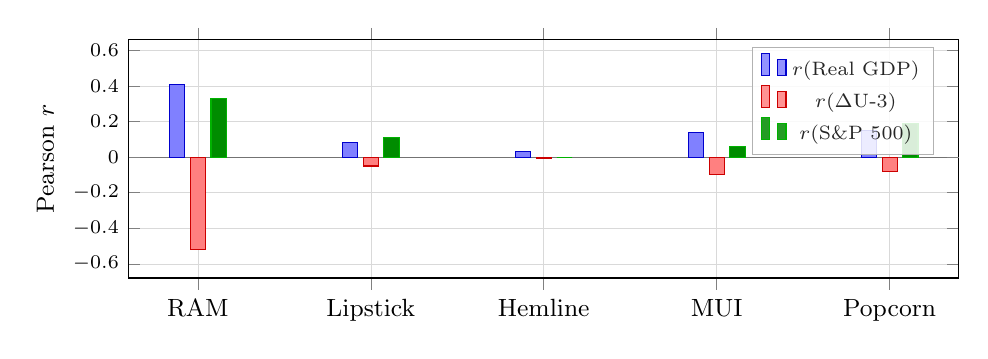
\begin{tikzpicture}
\begin{axis}[
  ybar,
  bar width=5.5pt,
  width=\linewidth, height=0.38\linewidth,
  ylabel={\small Pearson $r$},
  ymin=-0.68, ymax=0.66,
  xtick=data,
  symbolic x coords={RAM,Lipstick,Hemline,MUI,Popcorn},
  xticklabel style={font=\small},
  yticklabel style={font=\scriptsize},
  ytick={-0.6,-0.4,-0.2,0,0.2,0.4,0.6},
  grid=major, grid style={line width=0.2pt, draw=gray!30},
  extra y ticks={0},
  extra y tick labels={},
  extra y tick style={grid=major, grid style={black!55, thin}},
  legend pos=north east,
  legend style={font=\scriptsize, fill=white, fill opacity=0.85, draw=gray!60},
  clip=false,
]
\addplot[fill=blue!50, draw=blue!80!black] coordinates {
  (RAM,0.41)(Lipstick,0.08)(Hemline,0.03)(MUI,0.14)(Popcorn,0.15)
};
\addlegendentry{$r(\text{Real GDP})$}
\addplot[fill=red!50, draw=red!80!black] coordinates {
  (RAM,-0.52)(Lipstick,-0.05)(Hemline,-0.01)(MUI,-0.10)(Popcorn,-0.08)
};
\addlegendentry{$r(\Delta\text{U-3})$}
\addplot[fill=green!55!black, draw=green!70!black] coordinates {
  (RAM,0.33)(Lipstick,0.11)(Hemline,0.00)(MUI,0.06)(Popcorn,0.19)
};
\addlegendentry{$r(\text{S\&P 500})$}
\end{axis}
\end{tikzpicture}
\caption{Pearson correlations of the Ramification Index (RAM) and four folk indices against three macroeconomic variables, 1980--2026. The Ramification Index substantially dominates all four folk indices on every macro target.}
\label{fig:correlations}
\end{figure}

\section{Discussion}\label{sec:discussion}

The Ramification Index is a \emph{strictly better folk index}: it outperforms each incumbent consumer-behaviour proxy on coverage, timing, and correlation with macroeconomic truth. More importantly, it is not vulnerable to the kinds of behavioural shocks (pandemic, fashion fragmentation, athleisure, streaming) that have embarrassed the consumer-goods indices since 2020.

Three caveats apply. First, DRAM pricing reflects the decisions of a three-firm oligopoly; it is a signal of \emph{their} capex posture, not an independent clearing price. Antitrust authorities in the EU, US and China have found evidence of coordinated supply restraint in 2018--19. Second, generation transitions (DDR3 $\rightarrow$ 4 $\rightarrow$ 5; HBM2 $\rightarrow$ 3 $\rightarrow$ 3e) create compositional breaks in the nominal \$/GB series. Third, AI capex has begun to decouple HBM pricing from commodity DRAM; as HBM becomes a larger share of DRAM revenue, the Ramification Index may need to split into Commodity and AI sub-indices.

None of these caveats attaches to the incumbent folk indices, because those never claimed econometric validity. They are, as one of the sources of this paper put it, ``a good story with no real-world value'' \citep{baardwijk2010}. The Ramification Index aspires to be something stronger.

\section{Conclusion}\label{sec:conclusion}

The Lipstick, Hemline, Men's Underwear and Buttered Popcorn Indices are cultural fossils of a moment when economics borrowed from consumer behaviour because it had no faster indicator to hand. The memory industry now provides one.

We propose the \textbf{Ramification Index} as the natural twenty-first-century folk index. The name is a commitment. In algebraic number theory, a prime ramifies when it loses its primality and branches into factors as it passes into a larger field; the ramification index measures how completely that branching occurs. An economy is a field extension of its inputs: DRAM pricing is the prime that ramifies most completely, branching into server costs, AI compute budgets, consumer device prices, enterprise IT cycles, and ultimately GDP. The folk indices measure leaves at the end of those branches. The Ramification Index measures the root.

Its oligopoly structure, archival data, and rising macroeconomic weight make it harder to disrupt and better at what the older indices only claimed to do. The RAM in Ramification is not an accident. It never was.

\section*{Data availability}
All data used in this study are provided as a supplementary CSV (\verb|data/indices-wide.csv|). The interactive comparison dashboard is available at the companion repository.

\section*{Acknowledgements}
Thanks to the maintainers of the McCallum memory-price archive, AI Impacts, TrendForce, and NATO, and to the financial-journalism tradition that has kept the older indices alive long enough to be tested against modern data.

\section*{Competing interests}
The author declares no competing interests.

\bibliographystyle{unsrtnat}
\bibliography{references}

\end{document}
